\documentclass[unicode,11pt,a4paper,oneside,numbers=endperiod,openany]{scrartcl}
\usepackage{amsmath}
\usepackage{float}  % To prevent floating of figures
\usepackage{lmodern}
\usepackage{listings}
\usepackage{hyperref}
\usepackage[utf8]{inputenc}  % Allows UTF-8 input (for special characters, etc.)
\usepackage{amsmath}         % Provides advanced math features
\usepackage{amssymb}         % For additional math symbols
\usepackage{graphicx}        % Allows including images
\usepackage{array}           % For tables
\usepackage{geometry}        % To adjust page margins
\usepackage{hyperref}        % For links and references
\usepackage{fancyhdr}        % For customized headers and footers
\usepackage{multicol}        % For multiple columns
\usepackage{verbatim}        % For verbatim text (like the gene sequence)
\usepackage{longtable}       % For long tables that span multiple pages
\usepackage{xcolor}          % For colored text (if needed)
\usepackage{listings}
\usepackage{dnaseq}         % For DNA sequences
\usepackage{amsmath}
\usepackage{float}  % To prevent floating of figures
\usepackage{lmodern}
\usepackage{listings}
\usepackage{pdfpages}
\usepackage{booktabs}  % Add this line to include the booktabs package

\usepackage{ifthen}
\usepackage[utf8]{inputenc}
\usepackage{graphics}
\usepackage{graphicx}
\usepackage{hyperref}

\pagestyle{plain}
\voffset -5mm
\oddsidemargin  0mm
\evensidemargin -11mm
\marginparwidth 2cm
\marginparsep 0pt
\topmargin 0mm
\headheight 0pt
\headsep 0pt
\topskip 0pt        
\textheight 255mm
\textwidth 165mm

\newcommand{\duedate} {}
\newcommand{\setduedate}[1]{%
\renewcommand\duedate {See iCorsi for due date}}
\newcommand\isassignment {false}
\newcommand{\setassignment}{\renewcommand\isassignment {true}}
\newcommand{\ifassignment}[1]{\ifthenelse{\boolean{\isassignment}}{#1}{}}
\newcommand{\ifnotassignment}[1]{\ifthenelse{\boolean{\isassignment}}{}{#1}}

\newcommand{\assignmentpolicy}{
\begin{table}[h]
\begin{center}
\scalebox{0.8} {%
\begin{tabular}{|p{0.02cm}p{16cm}|}
\hline
&\\
\multicolumn{2}{|c|}{\Large\textbf{HPC Lab ---  Submission Instructions}}\\
\multicolumn{2}{|c|}{\large\textbf{(Please, notice that following instructions are mandatory: }}\\
\multicolumn{2}{|c|}{\large\textbf{submissions that don't comply with, won't be considered)}}\\
&\\
\textbullet & Assignments must be submitted to \href{https://www.icorsi.ch}{iCorsi} (i.e. in electronic format).\\
\textbullet & Provide both executable package and sources (e.g. C/C++ files, Matlab). 
If you are using libraries, please add them in the file. Sources must be organized in directories called:\\
\multicolumn{2}{|c|}{\textit{Project\_number\_lastname\_firstname}}\\
& and  the  file must be called:\\
\multicolumn{2}{|c|}{\textit{project\_number\_lastname\_firstname.zip}}\\
\multicolumn{2}{|c|}{\textit{project\_number\_lastname\_firstname.pdf}}\\
\textbullet &  The TAs will grade your project by reviewing your project write-up, and looking at the implementation 
                 you attempted, and benchmarking your code's performance.\\

\textbullet & You are allowed to discuss all questions with anyone you like; however: (i) your submission must list anyone you discussed problems with and (ii) you must write up your submission independently.\\
\hline
\end{tabular}
}
\end{center}
\end{table}
}
\newcommand{\punkte}[1]{\hspace{1ex}\emph{\mdseries\hfill(#1~\ifcase#1{Points}\or{Points}\else{Points}\fi)}}


\newcommand\serieheader[6]{
\thispagestyle{empty}%
\begin{flushleft}

\includegraphics[width=0.4\textwidth]{usi_inf.png}
\end{flushleft}
  \noindent%
  {\large\ignorespaces{\textbf{#1}}\hspace{\fill}\ignorespaces{ \textbf{#2}}}\\ \\%
  {\large\ignorespaces #3 \hspace{\fill}\ignorespaces #4}\\
  \noindent%
  \bigskip
  \hrule\par\bigskip\noindent%
  \bigskip {\ignorespaces {\Large{\textbf{#5}}}
  \hspace{\fill}\ignorespaces \large \ifthenelse{\boolean{\isassignment}}{\duedate}{#6}}
  \hrule\par\bigskip\noindent%  \linebreak
 }

\makeatletter
\def\enumerateMod{\ifnum \@enumdepth >3 \@toodeep\else
      \advance\@enumdepth \@ne
      \edef\@enumctr{enum\romannumeral\the\@enumdepth}\list
      {\csname label\@enumctr\endcsname}{\usecounter
        {\@enumctr}%%%? the following differs from "enumerate"
	\topsep0pt%
	\partopsep0pt%
	\itemsep0pt%
	\def\makelabel##1{\hss\llap{##1}}}\fi}
\let\endenumerateMod =\endlist
\makeatother




\usepackage{textcomp}





\begin{document}


\setassignment

\serieheader{High-Performance Computing Lab}{Institute of Computing}{Student: Jonatan Bella}{Discussed with: None}{Solution for Project 3}{}
\newline

\assignmentpolicy
This project will introduce you a parallel space solution of a nonlinear PDE using OpenMP.

% -------------------------------------------------------------------------- %
% -------------------------------------------------------------------------- %
% ---------------------- Exercise 1 -----------------------------------------%
% -------------------------------------------------------------------------- %
% -------------------------------------------------------------------------- %

\section{Task: Implementing the linear algebra functions and the stencil operators [35 Points]}

% -------------------------------------------------------------------------- %
% -------------------------------------------------------------------------- %
% ---------------------- Exercise 2 -----------------------------------------%
% -------------------------------------------------------------------------- %
% -------------------------------------------------------------------------- %
\subsection{Implement the missing linear algebra functions in linalg.cpp:}
\subsubsection{Norm 2}
For this implementation, I took advantage of the dot product function already implemented $hpc_dot$.
\begin{lstlisting}[language=C]
  double hpc_norm2(Field const& x, const int N) {
    double result = 0;
    result = hpc_dot(x,x,N);
    return sqrt(result);
}
\end{lstlisting}  
Since we can think of the L2 norm as the inner product of a vector with itself.
\subsubsection{Fill}
I used a simple for loop to set the entries in a vector to a value.
\begin{lstlisting}[language=C]
  void hpc_fill(Field& x, const double value, const int N) {
    for (int i = 0; i < N; i++){
        x[i] = value;
    }
}
\end{lstlisting}  
\subsubsection{axpy}
\begin{lstlisting}[language=C]
  void hpc_axpy(Field& y, const double alpha, Field const& x, const int N) {
    for (int i = 0; i < N; i++){
        y[i] += alpha * x[i];
    }
}
\end{lstlisting}  
This function iterates over the vectors and adds the scaled vector $x$ to $y$.
\subsubsection{add scaled diff}
\begin{lstlisting}[language=C]
void hpc_scaled_diff(Field& y, const double alpha, Field const& l,
                     Field const& r, const int N) {
    for (int i = 0; i < N; i++){
        y[i] = alpha * (l[i]-r[i]);
    }
}
\end{lstlisting}  
This function iterates over the vectors and adds the scaled difference of $l$ and 
$r$ to $x$ and stores the result in $y$.

\subsubsection{scale}
\begin{lstlisting}[language=C]
void hpc_scale(Field& y, const double alpha, Field const& x, const int N) {
    for (int i = 0; i < N; i++){
        y[i] = alpha * x[i];
    }
}
\end{lstlisting}  

\subsubsection{Linear Combination}
\begin{lstlisting}[language=C]
void hpc_lcomb(Field& y, const double alpha, Field const& x, const double beta,
               Field const& z, const int N) {
    for (int i = 0; i < N; i++){
        y[i] = alpha * x[i] + beta * z[i];
    }
}
\end{lstlisting} 
This function iterates over the vectors and adds the scaled vector $x$ (by alpha) to the scaled vector $z$ 
(by beta) and stores the result in $y$.

\subsubsection{Copy}
\begin{lstlisting}[language=C]
void hpc_copy(Field& y, Field const& x, const int N) {
    for (int i = 0; i < N; i++){
        y[i] = x[i];
    }
}
\end{lstlisting} 
This function iterates over the vectors and copies the vector $x$ to $y$.

\subsection{Implement the missing stencil kernel in operators.cpp:}
The stencil kernel fragment for the interior points is implemented as follows:
\begin{lstlisting}[language=C]
  for (int j=1; j < jend; j++) {
    for (int i=1; i < iend; i++) {
        f(i,j) = -(4. + alpha) * s_new(i,j)
               + s_new(i-1,j) + s_new(i+1,j)
               + s_new(i,j-1) + s_new(i,j+1)
               + beta * s_new(i,j) * (1.0 - s_new(i,j))
               + alpha * s_old(i,j);
    }
}
\end{lstlisting}
Following the equation as presented in the assignment. Notice that since we are not 
in the boundary, we can use directly the adjacent $s$ values. 

\subsection{Results}
Finally, I ran the program with the functions implemented before with the provided parameters: 
\begin{lstlisting}[language=bash]
  ./main 128 100 0.005
\end{lstlisting}
Using the node in an exclusive manner, with the following results: 

\begin{figure}[H]
  \centering
  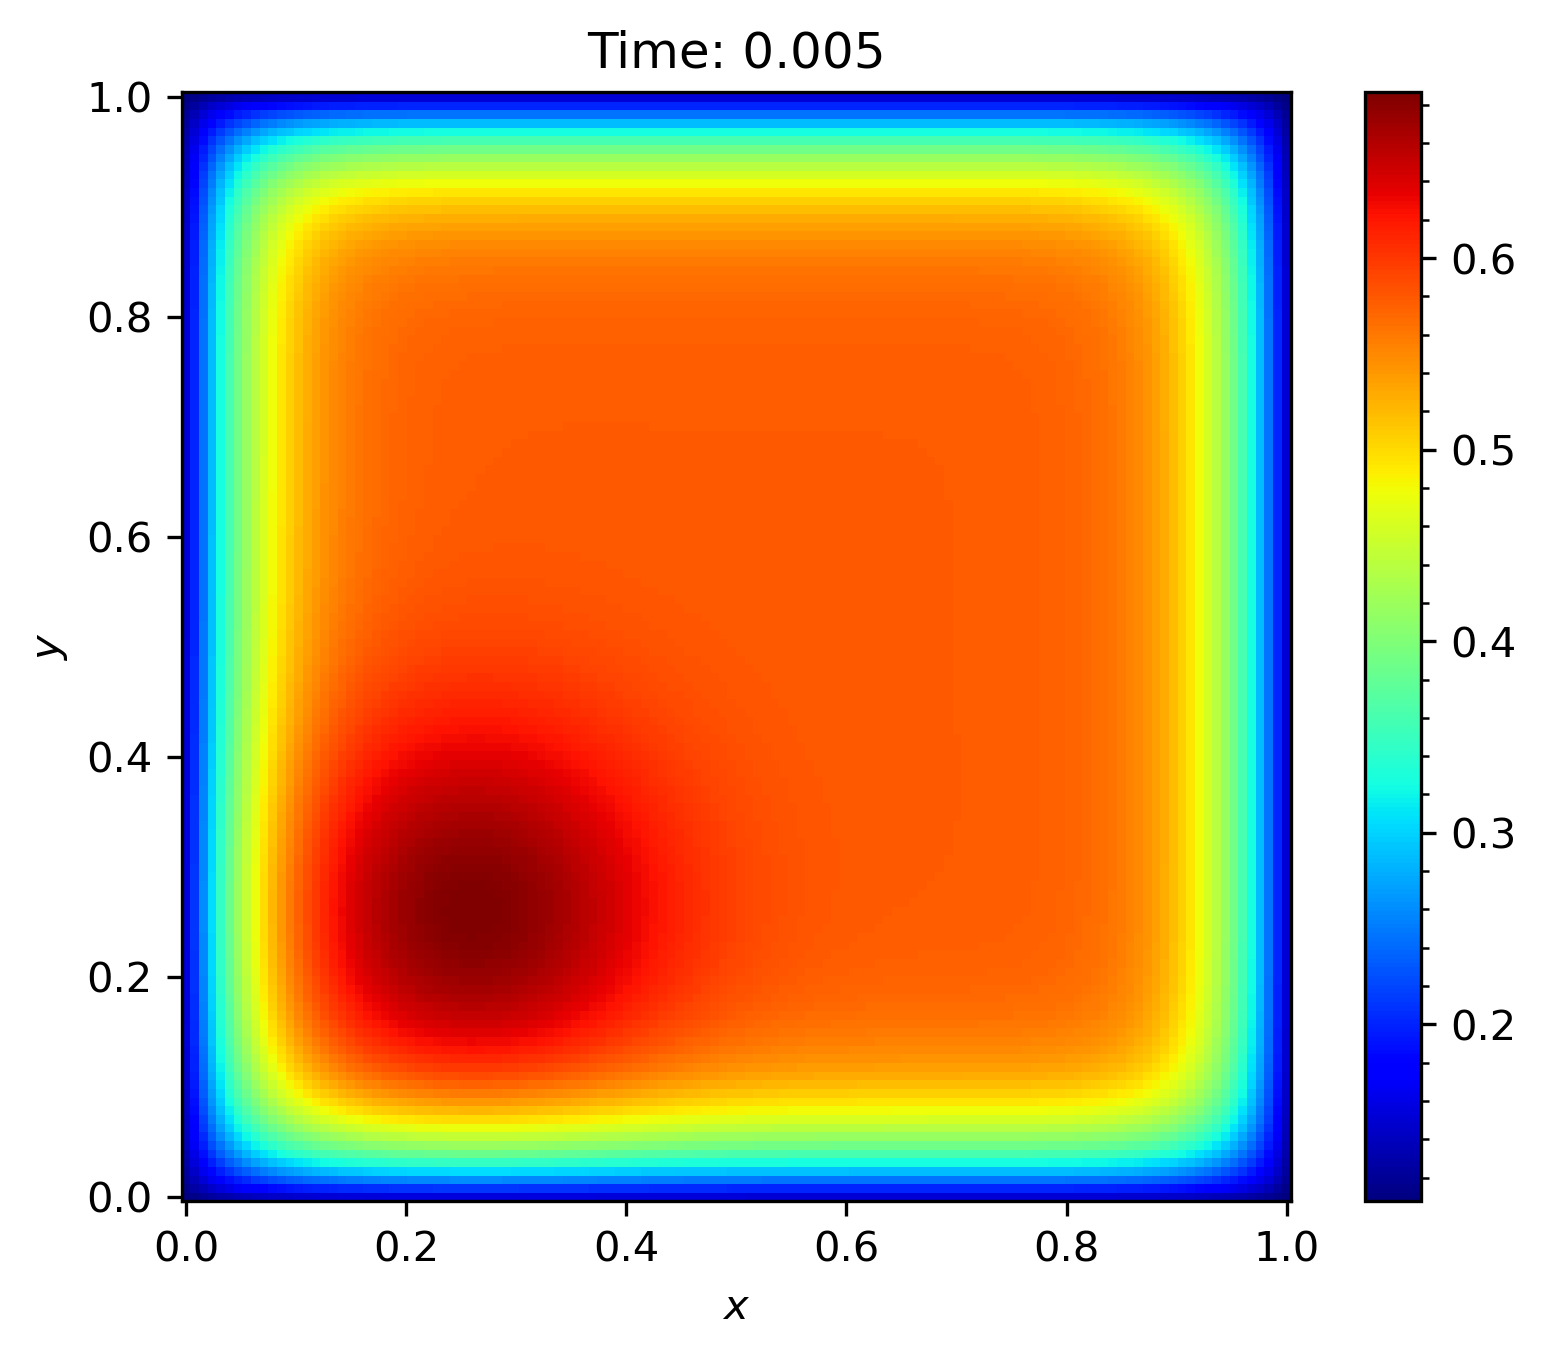
\includegraphics[width=0.7\textwidth]{./img/exe1/output.png}
  \caption{Contour plot of our simulation}
\end{figure}

\section{Task:  Adding OpenMP to the nonlinear PDE mini-app [50 Points]}
\subsection{Welcome message OpenMP}
To print out the number of threads used if OpenMP is enabled, I implemented the following code:
\begin{lstlisting}[language=C]
#ifdef _OPENMP
threads = omp_get_max_threads();
std::cout << "version   :: C++ OpenMP" << std::endl;
std::cout << "threads   :: " << threads << std::endl;
#else
std::cout << "version   :: C++ Serial" << std::endl;
#endif
\end{lstlisting}
Following the suggestions of the assignment with the use of macros.
Such that we get the number of maximum threads with the function $omp_get_max_threads()$ if
OPENMP is enabled. Otherwise, we print out that the program is running in serial.

\subsection{Parallelize the linear algebra functions}
In general, Almost all the function can be parallelized straightforwardly with the use of OpenMP in
this case. With the exception of the dot product one since it can lead to race conditions given that the 
variable $result$ is updated in parallel and accumulated. To solve this, we use the reduction clause in the 
parallel region.

\subsubsection{Dot product OPENMP directive}
\begin{lstlisting}[language=C]
#pragma omp parallel for default(none) shared(x,y,N) reduction(+:result)
\end{lstlisting}
As mentioned before, the dot product implementation can lead to a race condition
if we do not manage the shared variable $result$ properly. To solve this, we use the reduction clause.
In addition, as suggested in class, I use the default(none) clause to make sure that all the variables are
declared in the parallel region as a good practice. Therefore, we need to share the read variables $x$, $y$ and $N$.

\subsubsection{L2 norm}
No changes since the function calls for $hpc_dot$ which is already parallelized.

\subsubsection{Fill}
\begin{lstlisting}[language=C]
#pragma omp parallel for default(none) shared(x,value,N)
\end{lstlisting}
There is no possible raze condition since we are not updating the same variable in parallel.
I share the corresponding used variables. 

\subsubsection{axpy}
\begin{lstlisting}[language=C]
#pragma omp parallel for default(none) shared(alpha,x,y,N)
\end{lstlisting}
Same reason as the fill function, no race condition since 
the "accumulation" corresponds to the same iteration. Such that 
the updates are independent.
I share the corresponding used variables. 

\subsubsection{add scaled diff}
\begin{lstlisting}[language=C]
#pragma omp parallel for default(none) shared(alpha,x,y,N,l,r)
\end{lstlisting}

\subsubsection{scale diff}
\begin{lstlisting}[language=C]
#pragma omp parallel for default(none) shared(alpha,x,y,N)
\end{lstlisting}

\subsubsection{Linear Combination}
\begin{lstlisting}[language=C]
#pragma omp parallel for default(none) shared(alpha,x,y,N,beta,z)
\end{lstlisting}

\subsubsection{Copy}
\begin{lstlisting}[language=C]
#pragma omp parallel for default(none) shared(x,y,N)
\end{lstlisting}

\subsection{Operators.cpp parallelization}
The parallelization of the operators.cpp file is also straightforward since we can parallelize each of the 
stencil kernel fragments (that have a loop) without any risk of a race condition since there are no accumulation 
ongoing for the defined variables. 
Therefore, we can share all variables that are needed on each for loop, except the indices of the 
loop that are managed by the pragma directive.
\subsubsection{Interior points}
\begin{lstlisting}[language=C]
  #pragma omp parallel for default(none) shared(f,s,alpha,beta,y_old,jend,iend) 
  collapse(2)
\end{lstlisting}
In this case, we can use the collapse clause to collapse the two loops into one. \footnote{\url{https://stackoverflow.com/questions/13357065/how-does-openmp-handle-nested-loops}}
Which allow us to parallelize both loops, outer and inner ones.

\subsubsection{East boundary}
\begin{lstlisting}[language=C]
  #pragma omp parallel for default(none) 
  shared(alpha,beta,s_old,s_new,f,jend,bndE,i)
\end{lstlisting}
In this case, and the same for the next ones, is a simple for loop parallelization without
potential race conditions. We need to share the respective used variables given that we are using
default(none) clause.
\subsubsection{West boundary}
\begin{lstlisting}[language=C]
  #pragma omp parallel for default(none) 
  shared(alpha,beta,s_old,s_new,f,jend,bndW,i)
\end{lstlisting}
\subsubsection{North boundary}
\begin{lstlisting}[language=C]
  #pragma omp parallel for default(none) 
  shared(alpha,beta,s_old,s_new,f,iend,bndN,j)
\end{lstlisting}
\subsubsection{South boundary}
\begin{lstlisting}[language=C]
  #pragma omp parallel for default(none) 
  shared(alpha,beta,s_old,s_new,f,iend,bndS,j)
\end{lstlisting}

\subsection{Bitwise identical results}
In relation to this, and following the openmp specification \footnote{\url{https://www.openmp.org/spec-html/5.2/openmpsu50.html}},we can say that
it is practically challenging to obtain bitwise identical results. This happens since the order on which the values are combined are unspecified and
 different rounding errors may be introduced when dissimilar-sized values are joined in a different order.
Therefore, there is a trade-off in enforcing some ordering against parallel efficiency. However, slight variations provided by floating point operations 
and ordering of operations can be acceptable, even more if the difference on running time is substantial. 

\subsection{Strong Scaling}
\begin{figure}[H]
  \centering
  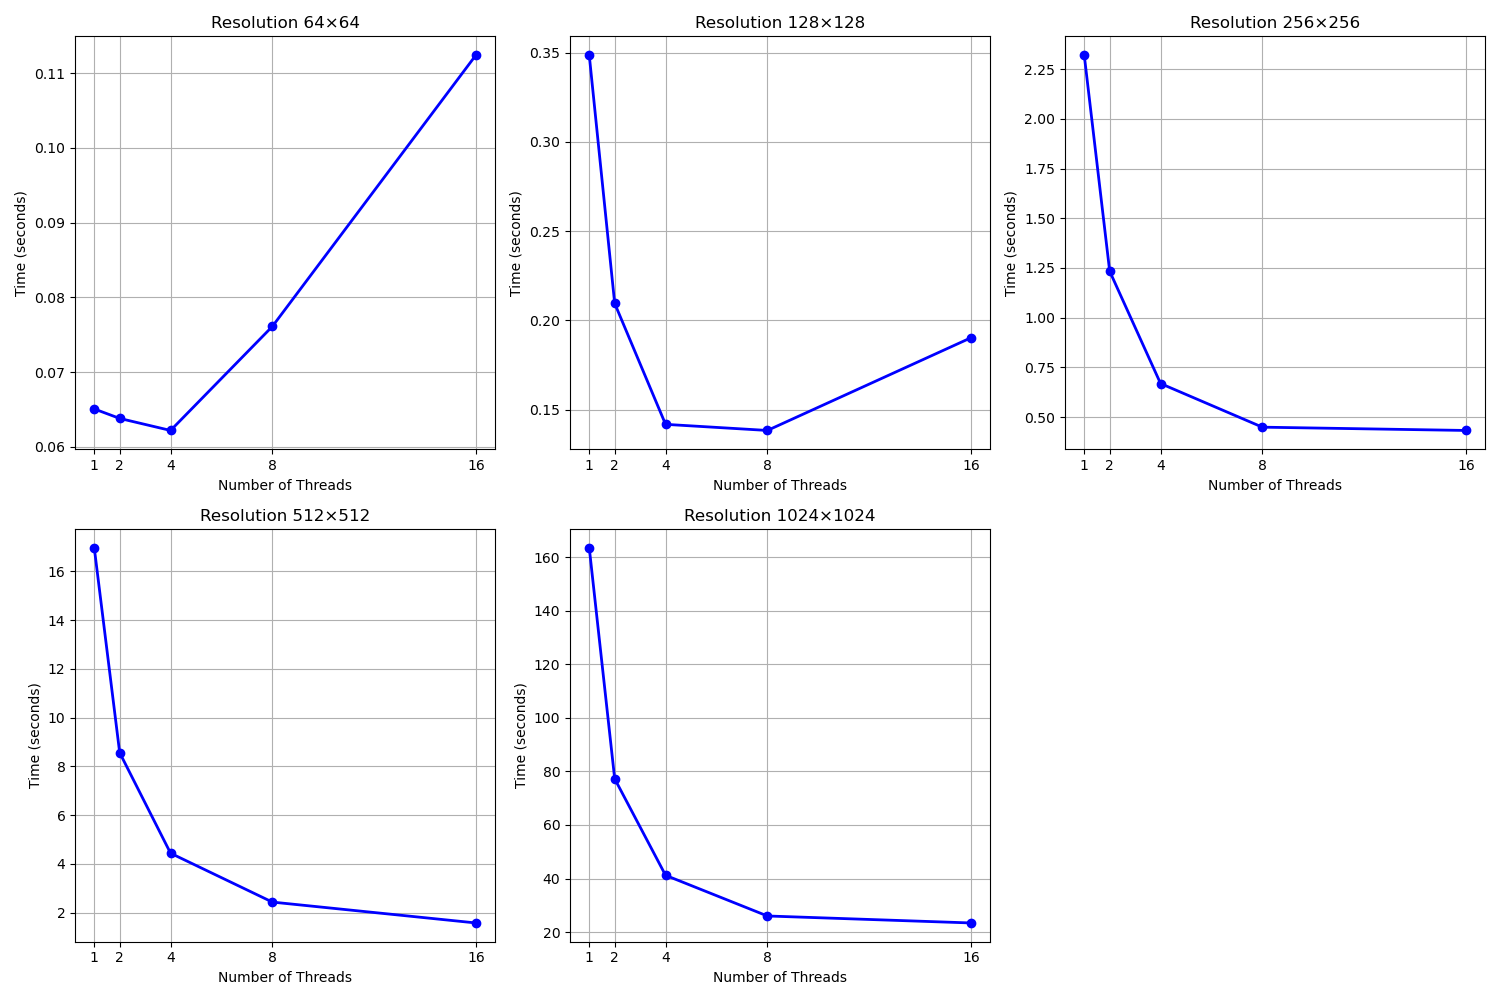
\includegraphics[width=\textwidth]{./img/exe2/strong_scaling.png}
  \caption{Strong scaling plot for each resolution and thread number}
\end{figure}

As we can see, there a substantial and increasing improvement relative 
to the amount of data processed. For example, the parallelization can have a small 
benefit or even negative effect if the size of the problem is small enough to not 
compensate for the overhead costs of the parallelization as it happen with $64$x$64$
example. 

\begin{table}[h!]
    \centering
    \caption{Scaling Analysis for Resolution 64$\times$64}
    \begin{tabular}{cccc}
        \toprule
        Threads & Time (s) & Speedup & Efficiency \\
        \midrule
        1  & 0.065 & 1.000 & 1.000 \\
        2  & 0.064 & 1.020 & 0.510 \\
        4  & 0.062 & 1.046 & 0.262 \\
        8  & 0.076 & 0.855 & 0.107 \\
        16 & 0.112 & 0.579 & 0.036 \\
        \bottomrule
    \end{tabular}
\end{table}

However, the benefits of the parallelization increased with the size. "Diluting" 
more the overhead costs. Justifying higher threads numbers. You can notice more in detail 
the improvement in efficiency and Speedup:

\begin{table}[h!]
    \centering
    \caption{Scaling Analysis for Resolution 128$\times$128}
    \begin{tabular}{cccc}
        \toprule
        Threads & Time (s) & Speedup & Efficiency \\
        \midrule
        1  & 0.349 & 1.000 & 1.000 \\
        2  & 0.210 & 1.663 & 0.832 \\
        4  & 0.142 & 2.458 & 0.614 \\
        8  & 0.138 & 2.519 & 0.315 \\
        16 & 0.190 & 1.832 & 0.114 \\
        \bottomrule
    \end{tabular}
\end{table}

\begin{table}[h!]
    \centering
    \caption{Scaling Analysis for Resolution 256$\times$256}
    \begin{tabular}{cccc}
        \toprule
        Threads & Time (s) & Speedup & Efficiency \\
        \midrule
        1  & 2.320 & 1.000 & 1.000 \\
        2  & 1.233 & 1.881 & 0.941 \\
        4  & 0.668 & 3.471 & 0.868 \\
        8  & 0.449 & 5.168 & 0.646 \\
        16 & 0.433 & 5.365 & 0.335 \\
        \bottomrule
    \end{tabular}
\end{table}

\begin{table}[h!]
    \centering
    \caption{Scaling Analysis for Resolution 512$\times$512}
    \begin{tabular}{cccc}
        \toprule
        Threads & Time (s) & Speedup & Efficiency \\
        \midrule
        1  & 16.974 & 1.000 & 1.000 \\
        2  & 8.560  & 1.983 & 0.991 \\
        4  & 4.436  & 3.826 & 0.957 \\
        8  & 2.432  & 6.980 & 0.873 \\
        16 & 1.575  & 10.775 & 0.673 \\
        \bottomrule
    \end{tabular}
\end{table}

\begin{table}[h!]
    \centering
    \caption{Scaling Analysis for Resolution 1024$\times$1024}
    \begin{tabular}{cccc}
        \toprule
        Threads & Time (s) & Speedup & Efficiency \\
        \midrule
        1  & 163.546 & 1.000 & 1.000 \\
        2  & 77.248  & 2.117 & 1.059 \\
        4  & 41.202  & 3.969 & 0.992 \\
        8  & 26.020  & 6.285 & 0.786 \\
        16 & 23.414  & 6.985 & 0.437 \\
        \bottomrule
    \end{tabular}
\end{table}

Notice that for obtaining this results I constructed a bash file ($strong\_scaling.sh$)
to automate the process of running the program with the different resolutions and 
thread numbers. An important remark is that I used the exclusive node in the 
$sbatch$ file to ensure that the whole node is used by the program, otherwise, the 
results would seem as that the parallelization would not be helping.

\subsection{Weak Scaling}
\begin{figure}[H]
  \centering
  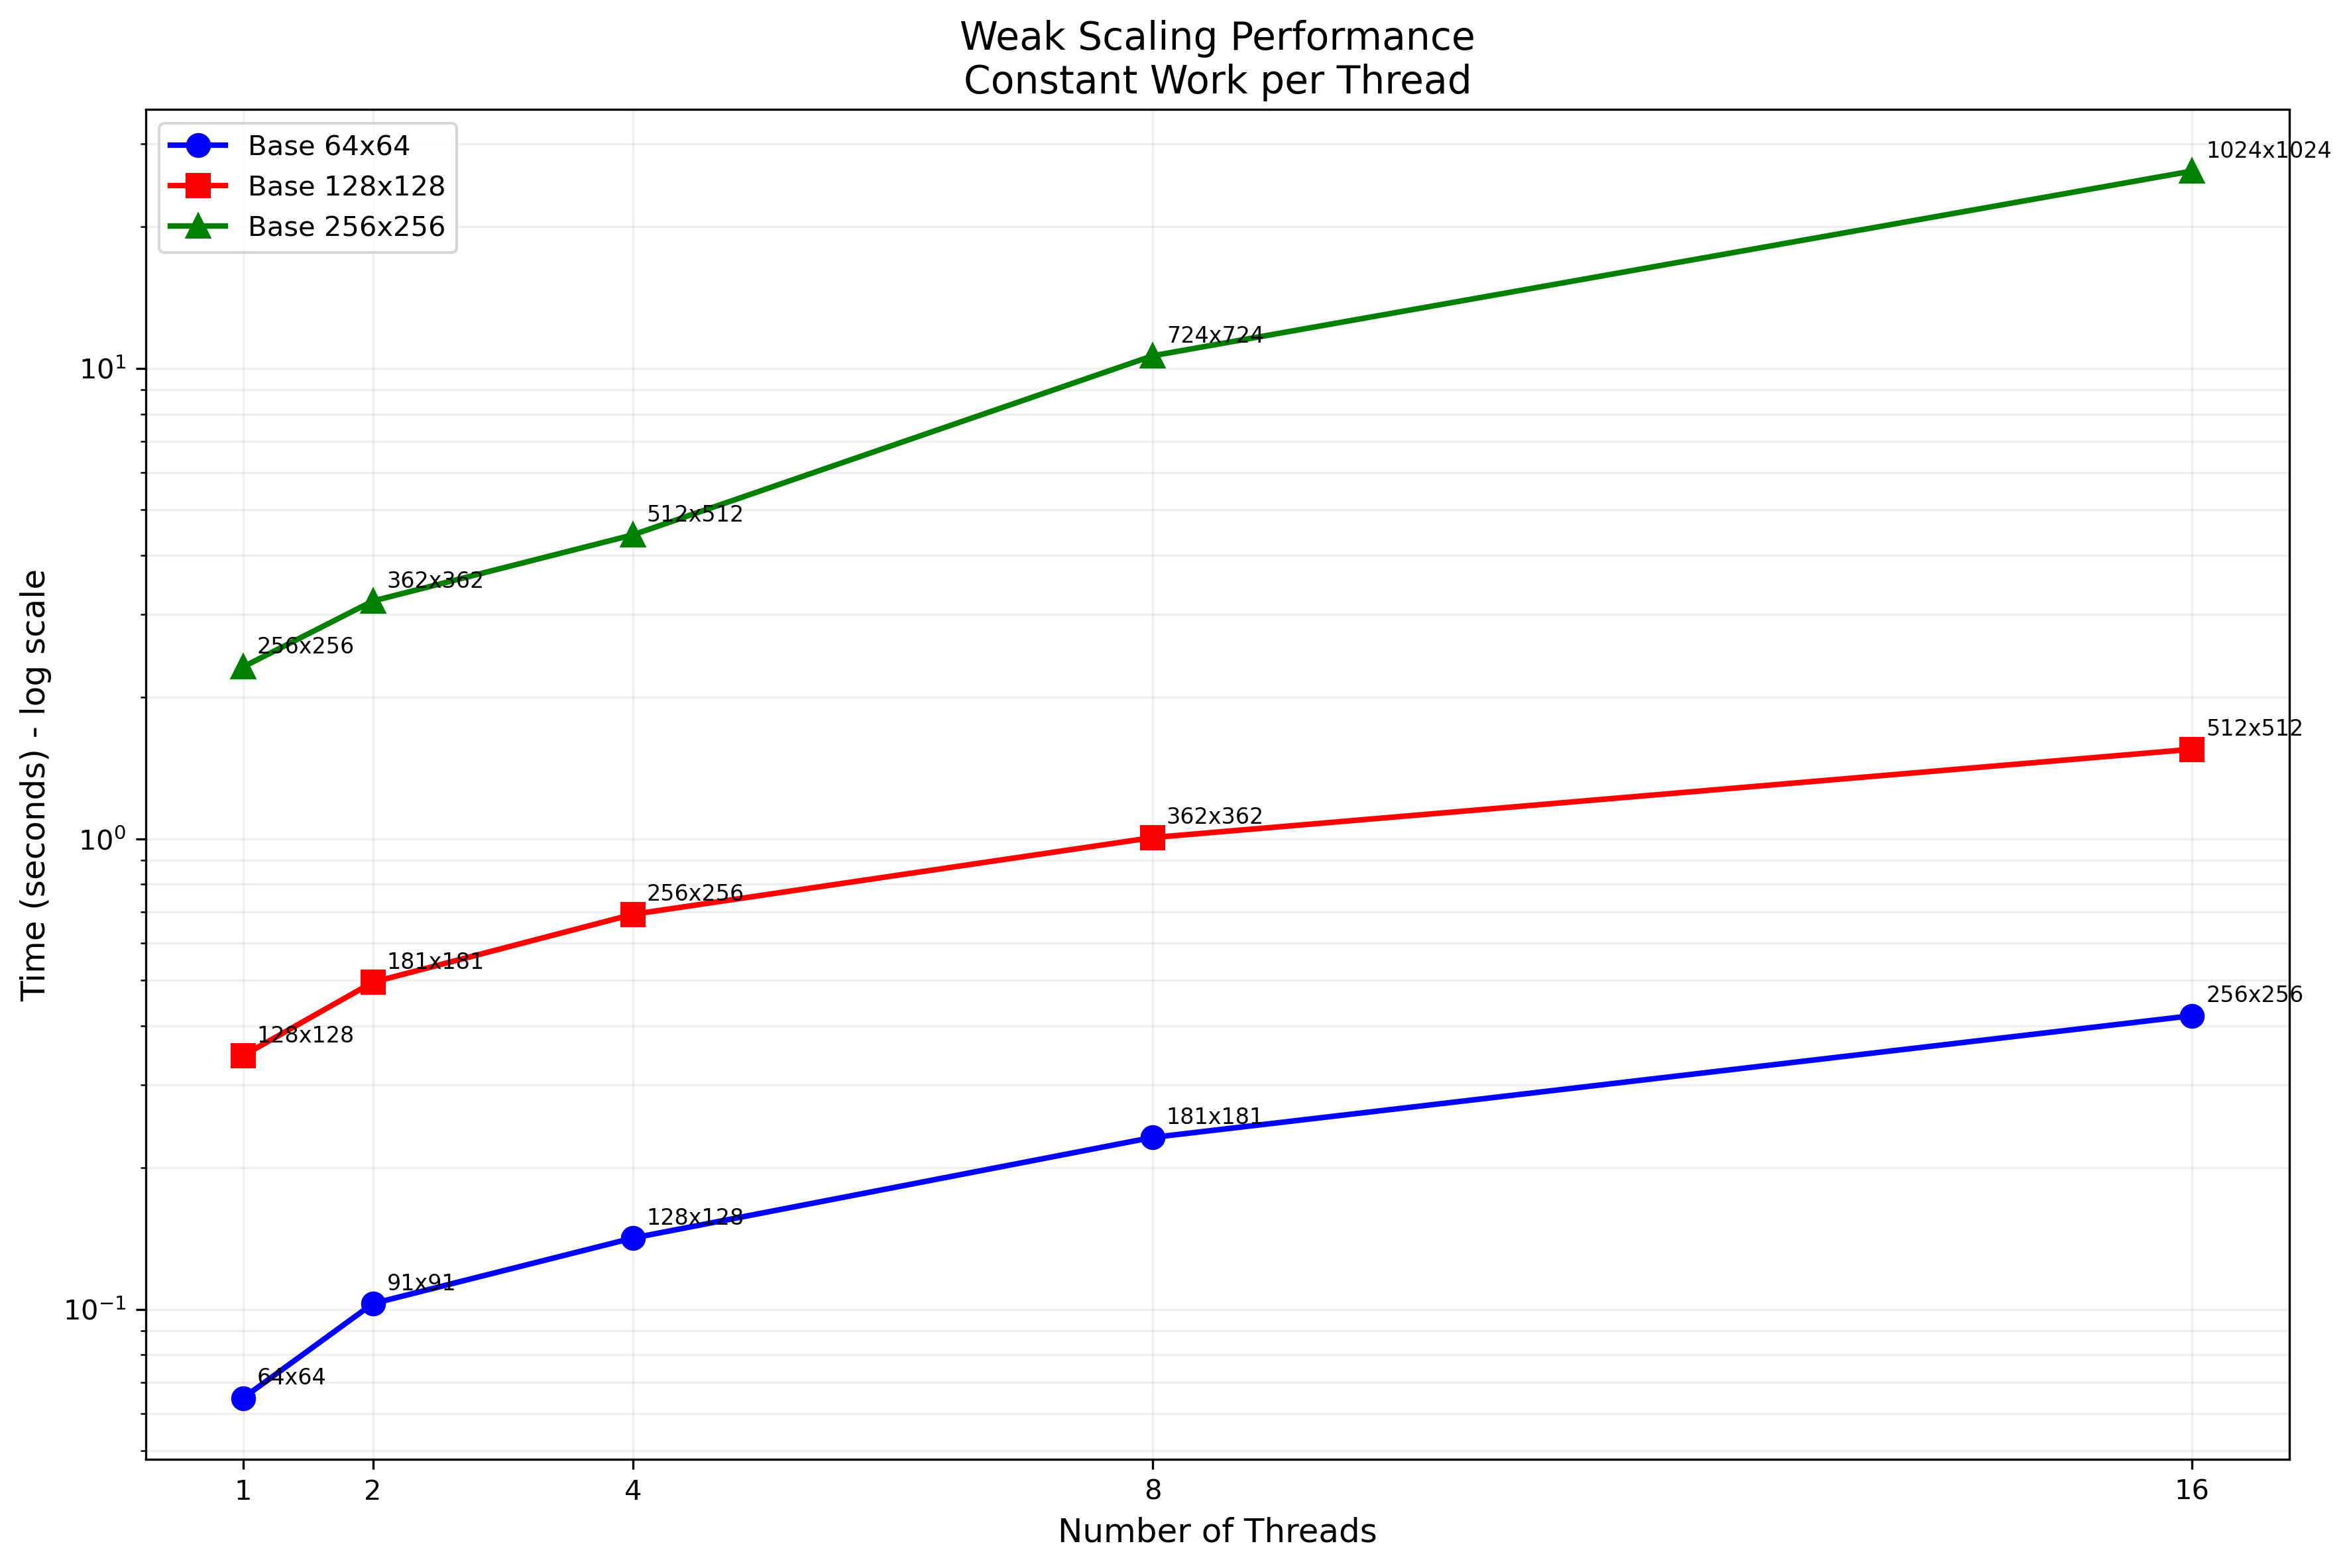
\includegraphics[width=\textwidth]{./img/exe2/weak_scaling.png}
  \caption{Weak scaling plot for a constant work per thread}
\end{figure}

Given a base size, we compute the size that keep the work per thread, with the increased
number of thread, constant:
\begin{itemize}
  \item Base 64: ~4100 work per thread
  \item Base 128: ~16400 work per thread
  \item Base 256: ~65600 work per thread
\end{itemize}

In an idea situation we would expect that doubling the threads and the grid size 
would stay roughly constant because each thread would handle the extra work. However, 
each thread adds an overhead cost since each thread share variables, needs to synchronize 
in reductions, etc. 

To implement this I modify the previous batch file ($weak\_scaling.sh$) to compute the 
grid size based on the work per thread and the base initial grid size such that it keeps the 
work per thread constant with the provided expression. Initially I tried to use the $sqrt$ of the number of threads, but 
it was not working as expected. \footnote{\url{https://www.unix.com/unix-for-dummies-questions-and-answers/152680-sqrt-bash.html}
\newline
\url{https://stackoverflow.com/questions/12722095/how-do-i-use-floating-point-arithmetic-in-bash}
\newline
\url{https://ryanstutorials.net/bash-scripting-tutorial/bash-functions.php}
}
Therefore, I made use of cases with precomputed square root values \footnote{\url{https://linuxize.com/post/bash-case-statement/}}

\section{Task:  Quality of the Report   [15 Points]}



\section*{Additional notes and submission details}
Submit the source code files (together with your used \texttt{Makefile}) in
an archive file (tar, zip, etc.) and summarize your results and the
observations for all exercises by writing an extended Latex report.
Use the Latex template from the webpage and upload the Latex summary
as a PDF to \href{https://www.icorsi.ch}{iCorsi}.

\begin{itemize}
\item Your submission should be a gzipped tar archive, formatted like project\_number\_lastname\_firstname.zip or project\_number\_lastname\_firstname.tgz. 
      It should contain:
  \begin{itemize}
    \item all the source codes of your OpenMP solutions.
    \item your write-up with your name  project\_number\_lastname\_firstname.pdf, 
  \end{itemize}
   \item Submit your .tgz through Icorsi.
  \end{itemize}


\end{document}
